\subsection{Сборка и запуск}
\subsubsection{Сборка проекта CFDCourse}

Описанная ниже процедура собирает проект в отладочной конфигурации.
Для проведения необходимых модификаций для сборки релизной версии смотри \ref{sec:release-build}.

\subsubsubsection{Подготовка}
\label{sec:install-prep}
\begin{enumerate}
\item
Для сборки проекта необходимо установить \ename{git} и \ename{cmake>=3.0}

В Windows необходимо скачать и установить диструбутивы:
\begin{itemize}
\item
\url{https://github.com/git-for-windows/git/releases/download/v2.38.1.windows.1/Git-2.38.1-64-bit.exe}
\item
\url{https://github.com/Kitware/CMake/releases/download/v3.24.2/cmake-3.24.2-windows-x86\_64.msi}
\end{itemize}

При установке cmake проследите, что бы путь к \ename{cmake.exe} сохранился в системных путях.
Msi установщик спросит об этом в диалоге.

В {\bf линуксе} используйте менеджеры пакетов, предоставляемые вашим дистрибутивом.
Также проследите чтобы были доступны компиллятор \ename{g++} и отладчик \ename{gdb}.

\item
Создайте папку в системе для репозиториев. Например \ename{D:/git_repos/}

\item
Возьмите необходимые заголовочные библиотеки boost из \url{https://disk.yandex.ru/d/GwTZUvfAqPsZBQ}
и распакуйте архив в папку для репозиториев (D:/git\_repos/boost).
Проследите, чтобы внутри папки boost сразу шли папки с кодом (\ename{accumulators}, \ename{algorithm}, ...)
и заголовочные файлы (\ename{align.hpp}, \ename{aligned_storage.hpp}, ...)
без дополнительных уровней вложения.

\item
Откройте терминал (git bash в Windows).

\item
С помощью команды cd в терминале перейдите в папку для репозиториев
\begin{shelloutput}
> cd D:/git_repos
\end{shelloutput}

\item
Клонируйте репозиторий
\begin{shelloutput}
> git clone https://github.com/kalininei/CFDCourse24
\end{shelloutput}
В директории (\ename{D:/git_repos} в примере) появится папка \ename{CFDCourse24}, которая является корневой папкой проекта
\end{enumerate}

\subsubsubsection{VisualStudio}
\label{sec:vs-build}

\begin{enumerate}
\item
Cоздайте папку build в корне проекта СFDCourse24

\item
Скопируйте скрипт winbuild64.bat в папку build. Далее вносить изменения
только в скопированном файле.

\item
Скрипт написан для версии \ename{Visual Studio 2019}. Если используется другая версия,
измените в скрипте значение переменной \cvar{CMGenerator} на соответствующие вашей версии.
Значения для разных версий Visual Studio написаны ниже
\begin{shelloutput}
SET CMGenerator="Visual Studio 17 2022"
SET CMGenerator="Visual Studio 16 2019"
SET CMGenerator="Visual Studio 15 2017"
SET CMGenerator="Visual Studio 14 2015"
\end{shelloutput}

\item
Запустите скрипт \ename{winbuild64.bat} из папки \ename{build}. Нужен доступ к интернету.
В процессе будет скачано около 200Мб пакетов, поэтому первый запуск может занять время

\item
После сборки в папке \ename{build} появится проект \ename{VisualStudio} \ename{cfdcourse24.sln}.
Его нужно открыть в \ename{VisualStudio}.
Дерево решения должно иметь следующий вид:
\begin{center}
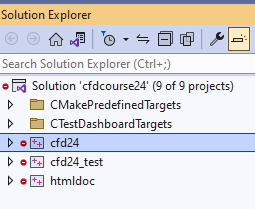
\includegraphics[width=0.3\linewidth]{vs_solution_explorer.png}
\end{center}
Проекты:
\begin{itemize}
\item \ename{cfd24} -- расчётная библиотека
\item \ename{cfd24_test} -- модульные тесты для расчётных функций
\end{itemize}

\item
Проект \ename{cfd24_test} необходимо назначить запускаемым проектом. Для этого нажать правой кнопкой мыши по проекту и в выпадающем меню
выбрать соответствующий пункт. После этого заголовок проекта должен стать жирным.
\begin{center}
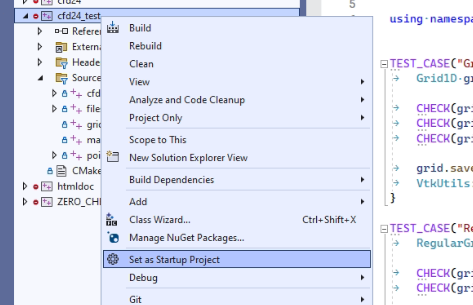
\includegraphics[width=0.5\linewidth]{win_startup_project.png}
\end{center}

\item
Скомпиллировать решение. Несколько способов:
\begin{itemize}
\item \ename{Ctrl+Shift+B},
\item \ename{Build->Build Solution} в основном меню,
\item \ename{Build Solution} в меню решения в дереве решения,
\item \ename{Build} в меню проекта \ename{cfd24_test}.
\end{itemize}

\item
Запустить тесты (проект \ename{cfd24_test}) нажав \ename{F5} (или кнопку отладки в меню).
После отработки должно высветиться сообщение об успешном прохождении всех тестов.

\item
Бинарные файлы будут скомпиллированы в папку \ename{CFDCourse24/build/bin/Debug}.
В случае работы через отладчик выходная директория, куда будут скидываться все файлы (в частности, vtk),
должна быть \ename{CFDCourse24/build/src/test/}.
\end{enumerate}

\subsubsubsection{VSCode}
\label{sec:vscode-build}

\begin{enumerate}
\item
Открыть корневую папку проека через \ename{File->Open Folder}
\item
Установить предлагаемые расширения cmake, c++
\item
Для настройки отладки создайте конфигурацию launch.json следующего вида
\begin{center}
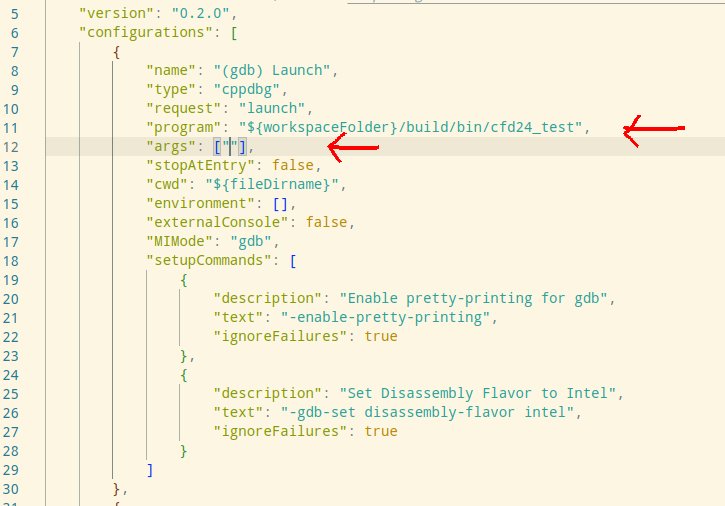
\includegraphics[width=0.7\linewidth]{vscode_launch_json.png}
\end{center}
\begin{itemize}
\item
Для этого перейдите в меню \ename{Run and Dubug} (\ename{Ctrl+Shift+D}), нажмите
\ename{create launch.json}, выберите пункт \ename{Node.js}.
\item
После этого в корневой папке появится файл \ename{.vscode/launch.json}.
\item
Откройте этот файл в \ename{vscode}, нажмите \ename{Add configuration}, \ename{(gdb) Launch} или \ename{(Windows) Launch} в зависимости от ОС.
\item
Далее напишите имя программы как показано на картинке.
\item
Используйте поле args для установки аргументов запуска.
\item
Выберите созданную конфигурацию для запуска отладчика по \ename{F5}
\begin{center}
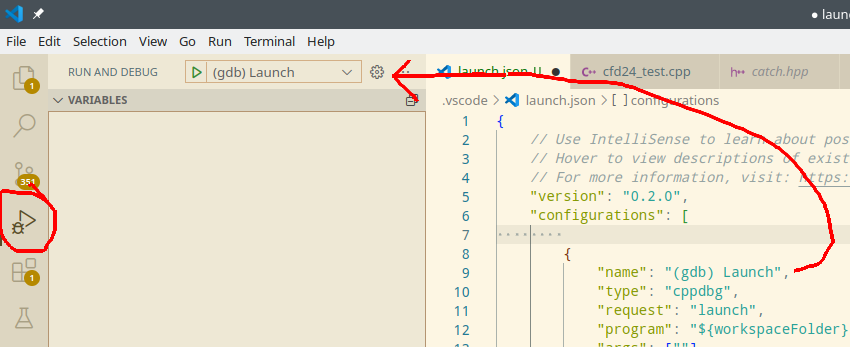
\includegraphics[width=0.7\linewidth]{vscode_launch.png}
\end{center}
\end{itemize}

На скриншотах представлены настройки в случае работы в линуксе. Для работы под виндоус 
\begin{shelloutput}
"name" : "(Windows) Launch",
"program": "${workspaceFolder}/build/bin/Debug/cfd24_test.exe"
\end{shelloutput}
\end{enumerate}

\subsubsection{Запуск конкретного теста}

По умолчанию программа \ename{cfd_test} прогоняет все объявленные в проекте тесты. Иногда может возникнуть необходимость
запустить только конкретный тест в целях отладки или проверки.
Для этого нужно передать программе аргумент с тегом для этого теста.

Тег для теста -- это второй аргумент в макросе \cvar{TEST_CASE}, записанный в квадратных скобках.
Добавлять нужно вместе со скобками. Например, \cvar{[ping]}.

Чтобы добавить аргумент в \ename{VisualStudio}, необходимо в контекстном меню проекта \ename{cfd_test} выбрать опции отладки
\begin{center}
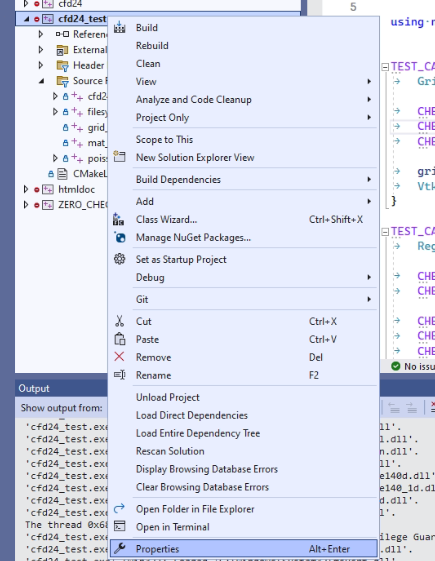
\includegraphics[width=0.7\linewidth]{win_debug_args_1.png}
\end{center}
и там в поле Аргументы прописать нужный тэг.
\begin{center}
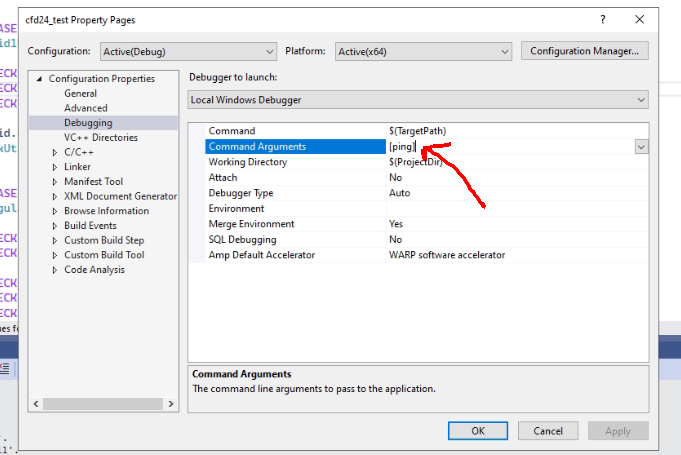
\includegraphics[width=0.9\linewidth]{win_debug_args_2.png}
\end{center}

В \ename{VSCode} аргументы нужно добавлять в файле \ename{.vscode/launch.json} в поле args в кавычках
(см. картинку \ref{sec:vscode-build} с настройками launch.json).

\subsubsection{Сборка релизной версии}
\label{sec:release-build}

Релизная сборка программ даёт многократное увеличение производительности,
но при этом отладка приложений в таком режиме невозможна.

{\bf Visual Studio}
\begin{enumerate}
\item Создать папку \ename{build-release} рядом с папкой \ename{build}.
\item Скопировать в неё файл \ename{winbuild64.bat} из папки \ename{build}. 
\item В скопированном файле произвести замену \cvar{Debug} на \cvar{Release}
\begin{shelloutput}
-DCMAKE_BUILD_TYPE=Release ..
\end{shelloutput}
\item Запустить \ename{winbuild64.bat} из новой папки
\item Открыть \ename{build-release/cfdcourse24.sln} в \ename{Visual Studio}
\item В проекте студии установить релизную сборку
\begin{center}
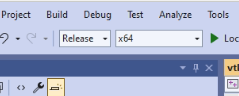
\includegraphics[width=0.5\linewidth]{release_build.png}
\end{center}
\item Это новое решение, не связанное настройками с \ename{debug}-версией.
      Поэтому нужно заново настроить запускускаемым проектом \ename{cfd_test}
      и, если нужно, настроить аргументы отладки.
\item Бинарные файлы будут скомпиллированы в папку \ename{CFDCourse24/build_release/bin/Release}.
      В случае работы через отладчик выходная директория -- \ename{CFDCourse24/build_release/src/test/}.
\end{enumerate}

{\bf VSCode}
\begin{enumerate}
\item Выбрать релизную сборку в \ename{build variant}
\item Нажать \ename{Build}
\item Нажать \ename{Launch}
\begin{center}
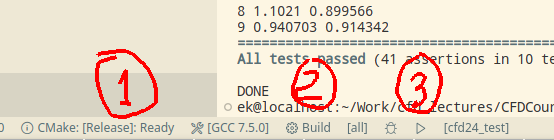
\includegraphics[width=0.5\linewidth]{release_build_2.png}
\end{center}
\end{enumerate}
